%% how will i tackle the problem with justifications 
%% based on ideas in BACKGROUND

\chapter{Implementation}\label{ch:impl}

\section{Using a MATLAB-based neural network as reference} \label{se:impl.matlab.nn}

There are several motivations for choosing this particular implementation of neural network as reference. First, MATLAB implementation is heavily reliant upon the mathematical interpretation of neural network and is clearly understandable where matrix multiplication and vectorisation is concerned. It was projected that it would be fairly simple and in the closest-in-spirit implementation to how it may work in Accelerate due to this.

Secondly, the MATLAB implementation had a certain data set with expected 'answers' to compare my own implementations to. Thus, I could be assured that my implementation in Accelerate was accurate enough to be reliable, particularly in the light of difficulty of debugging Accelerate programs. Passing this 'accuracy' test will prove the small network reliable enough to be built upon for further development in the future.

Thirdly, the codebase that I am basing my program is from Coursera, an online self-learning course, made by Andrew Ng of Stanford University. This course has drawn wide praise for its material and presumed to be reviewed by many in the same field. The structure of the course is reliable in terms of correctness and efficiency, and implemented already with much knowledge in the field. Hence, I projected that the MATLAB implementation would be optimised for the best performance.

Lastly, in terms of familiarity, I was more conversed with MATLAB than with other neural network implementations, such as Python, C++, or Haskell, (PUT REFERENCES TO THESE IMPLEMENTATIONS) which may needlessly increase the time to start the project. I had researched about other implementations, but found that it took more time to understand these in order to integrate or implement an Accelerate neural network.

TO CHECK::::: Can C++ or Python versions use multiple threads/GPU?

\subsection{Key differences from Accelerate} \label{se:impl.matlab.background}
%% or divide this up into implementation section

MATLAB, or Matrix Laboratory, is a highly doman-specific programming language, specialised to conduct numerical calculations and analysis. It was created in the 1970s, and is an imperative, object-orientated, procedural language. It is widely used among the industry and academia, particularly in science, engineering and economics.

MATLAB is a weakly typed programming language, as types are implicitly converted. This means that variables can be declared without an explicit declaration of their type~\cite{Wiki1}. Furthermore, MATLAB is also dynamically typed, meaning that the types may change during runtime. 

MATLAB functions automatically apply multiplications of a scalar term to a matrix, by applying the operation of the scalar to each element of the matrix. Thus, if \texttt{a} is a scalar and \texttt{xs} is a matrix, it is possible to simply do \texttt{a} $\times$ \texttt{xs}. In Accelerate, this would be \texttt{A.map (*a) xs}. As a result, MATLAB code is deceptively compact and does not reveal the actual structure of the underlying operation just by looking at the code. 

Other points include starting index of matrices and arrays being $1$, not $0$. Also, MATLAB method dispatching does not strictly adhere to the method signature, but selects the appropriate method by first matching the arguments in a class precedence and then by left-most priority~\cite{Mat17}. %MATLAB does not support overloading functions of the same name using different signature of the same name.

\section{Accelerate Implementation} \label{se:impl.acc}

\subsection{Neural network structure} \label{se:impl.nn.struct}

I have implemented a two-layered, fully connected simple neural network, with one hidden layer.

My implementation can easily be modified to take more than 1 hidden layer by changing the \texttt{nnCostFunction}. For instance, each extra hidden layer should only require implementing two extra matrix multiplications in feed-forward ad backpropagate parts, plus all the steps required to update the new theta layer calculations (see~\ref{fig:nnCostFunction.hiddenlayers}).

\begin{figure}
  \begin{lstlisting}
    -- current feed-forward with 1 hidden layer
    a3 :: Acc (Matrix Float)
    a1 = xs 
    z2 = theta1 <> transpose a1 
    a2 = (fill (lift (Z :. h :. constant  1)) 1 :: Acc (Matrix Float)) 
         A.++ (A.transpose $ A.map sigmoid z2) 
    z3 = a2 <> A.transpose theta2 
    a3 = A.map sigmoid z3
    
    -- an example feed-forward with 2 hidden layers
    a4 :: Acc (Matrix Float)
    a3' = (fill (lift (Z :. h' :. constant  1)) 1 :: Acc (Matrix Float))
          A.++ (A.transpose $ A.map sigmoid z3)
    z4 = a3' <> A.transpose theta3
    a4 = A.map sigmoid z4
    
    -- an example backpropagate with 2 hidden layers
    d4 = A.zipWith (-) a4 ys
    d3 = A.zipWith (*) 
         (d4 <> theta3)
         ((fill (lift (Z :. h' :. constant  1)) 1 :: Acc (Matrix Float)) 
           A.++ (A.transpose $ A.map sigmoidGradient z3)) 
    d2 = A.zipWith (*) 
         (d3 <> theta2)
         ((fill (lift (Z :. h :. constant  1)) 1 :: Acc (Matrix Float)) 
           A.++ (A.transpose $ A.map sigmoidGradient z2)) 
  \end{lstlisting}
  \caption{Changing the number of hidden layers in \texttt{nnCostFunction}}
  \label{fig:nnCostFunction.hiddenlayers}
\end{figure}

\subsection{Program structure} \label{se:impl.program.struct}

In terms of program structure, I closely followed the flow in the MATLAB version. It can be portioned into 3 parts: (1) initialisation; (2) neural network cost function; and, (3) function minimise conjugate gradient function. The implementation code is available at~\cite{McDJeo}.

\subsubsection{Initialisation} \label{se:impl.init}

Initialisation is a straightforward process. We initialise (1) the regularisation parameter \texttt{lambda}; (2) initial weight vectors, in this instance there are \texttt{theta1}, \texttt{theta2}; (3) size of the input, hidden, output layers; and, (4) the input training data set \texttt{xs} and the output vector \texttt{ys} to conduct the supervised learning. 

The number of input units correspond to the number of attributes in each sample of \texttt{xs}. The number of output units correspond to the number of classifications that these samples could be divided into, or, the range of the values of \texttt{ys}. Setting the number of neurons in the hidden layer is a bit of a mystery and seems to be done by trial-and-error. In \ref{se:res.testdata}, the hidden units are 25 neurons and 300 neurons for the two different handwritten numbers data sets and these are taken from other implementations with the same data sets, who had found these the most effective numbers by testing.

Matrix \texttt{xs} represents $m$ training set data. After it has been loaded, each row of \texttt{xs} should represent a single training example, $x_1, x_2, ..., x_m$ where the length of vector $x_i$ is the size of the input layer. A column vector of $1$s is added to the leftmost of the array to represent the bias neuron, as shown below.
\[
 \texttt{xs} =
    \begin{bmatrix}
      1 \\
      1 \\
      ... \\ 
      1
    \end{bmatrix}
    \begin{bmatrix}
       x_1 \\
       x_2 \\
       ... \\
       x_m
    \end{bmatrix}
\]

This is implemented in Accelerate using a combination of \texttt{fill} and concatenation \textbf{A.++}. Accelerate's operations are not the same as Haskell Prelude's, even if some operation names coincide. Thus they are distinguished by a prefix \texttt{A}, \texttt{P} for Accelerate and Prelude correspondingly, for instance \texttt{A.++} and \texttt{P.++}. Other key matrix manipulating functions used throughout the program include \texttt{A.take, A.drop, A.map} and \texttt{A.zipWith}.

An effectiveness of the random initialisation of weight vectors will influence the accuracy of the neural network. Initial values should be in the range $[-\epsilon_{init}, \epsilon_{init}]$~\cite{Ng12}. One popular choice of $\epsilon_{init}$ is,
\[ \epsilon_{init} = \sqrt{\frac{6}{L_{in} + L_{out}}} \]
where $L_{in}$ is number of units in the preceding layer, and $L_{out}$ is the number of units in the subsequent layer of the weight vector-in-question. 

Optimal regularisation parameter \texttt{lambda}, is also discovered by trial-and-error. It is set by the user to set the level of appropriate 'overfitting' of the neural network to the training set. Whether higher or lower overfitting to the training set is better or worse for making predictions on new samples, depends on the nature of the data. 

\subsubsection{Neural network cost function, \texttt{nnCostFunction}} \label{se:impl.nnCostFunction}

This function applies both the feed-forward and back-progapation to sample data inputs and updates the weight vectors and error costs accordingly. 

As described in \ref{sec:training} we apply the BGD method by grouping all the sample data into one massive batch to parse them in all at once for higher accuracy. 

As \texttt{nnCostFunction} is used in conjunction with \texttt{fmincg} function~\ref{se:impl.fmincg}, it was necessary to flatten all the weight vectors into one before passing into, and also out of the \texttt{nnCostFunction}. The fused vector is sliced and reshaped this its original shapes inside \texttt{nnCostFunction}, which is implemented using \texttt{reshape} as shown in~\ref{fig:reshape}.

\begin{figure}
	\begin{lstlisting}
	-- type of reshape
    reshape :: (Shape sh, Shape sh', Elt e) =>
                Exp sh -> Acc (Array sh' e) -> Acc (Array sh e)

    -- unroll theta1, theta2
    theta1 = reshape (index2 hiddenl (inputl +1)) $ A.take (hiddenl*(inputl+1)) thetas
    theta2 = reshape (index2 outputl (hiddenl+1)) $ A.drop (hiddenl*(inputl+1)) thetas
	\end{lstlisting}
  	\caption{Reshaping vectors into matrices in Accelerate.}
	\label{fig:reshape}
\end{figure}

\texttt{reshape} is tricky to maneuver at first, because it must be supplied with a \texttt{Exp sh}. \texttt{Exp sh} can be made in various ways and sometimes requires its type to be defined. For example, in the case where one \texttt{lift}s a \texttt{(Z:.m:.n)} form to supply \texttt{fill} with an \texttt{Exp sh},
$$\texttt{fill (lift (Z:.m:.n)) 1 :: Acc (Matrix Float)}$$
Thus, I found operations involving \texttt{Exp sh} quite tricky at times due to typing.

Matrix multiplications was initially implemented using \texttt{mmult}, but was eventually replaced with \texttt{hmatrix} package, which has a better performance. 

\subsubsection{Function minimise nonlinear conjugate gradient function, \texttt{fmincg}} \label{se:impl.fmincg}

This function repeats \texttt{nnCostFunction} for certain number of iterations, and progressively tries to minimise the error in the weight matrices. Generally, function minimisation by conjugate gradients is a quadratically convergent gradient method used to locate a local minimum when the function has several variables, or, is \textit{multivariate}~\cite{FleRee}.

In MATLAB, function minisation by conjugate gradient is a function called \texttt{fminunc}, which states that given a starting point \texttt{x0} (can be a scalar, vector or a matrix), \texttt{x} is the the local minimum of unconstrained function \texttt{func}~\cite{Mat17}:
$$\texttt{x = fminunc(func, x0)}$$
\texttt{fmincg} function is a modified version of \texttt{fminunc} and has the following MATLAB equation:
$$\texttt{function [X, fX, i] = fmincg(f, X, options, P1, P2, P3, P4, P5)}$$
According to the author, it is more efficient than \texttt{fminunc} in that it uses 'Polack-Ribiere' conjugate gradients, quadratic and cubic polynomial approximations and 'Wolfe-Powell stopping criteria' to more efficiently calculate slope and stepping sizes~\cite{Reb13}. The mathematics behind this method is beyond the scope of my understanding.

\texttt{fmincg} terminates when it either finds the local minimum, or if the progress is so insignificant that it is not worth any further exploration. It must be given a cost function \texttt{f}, initial weight vector \texttt{X} and maximum iteration number in \texttt{options}. Other parameters are not supplied. 

\texttt{fmincg} returns the solution vector as \texttt{X} and a cost vector as \texttt{fX}. \texttt{fX} starts off as an empty vector, and \texttt{fmincg} pushes the cost/error of the newly recalibrated weights in each iteration to the back of \texttt{fX}. The end result is that the caller to see progress made throughout the iterations upon checking \texttt{fX}. Other variables are discarded.

My Accelerate implementation of \texttt{fmincg} can be seen in~\ref{fig:fmincg}. The vector argument is a concatenation of flattened weight matrices and is fed into the function argument. This is to enable \texttt{fmincg} to execute the function indepedent of the structure of the underlying neural network, i.e. the number of hidden layers. It is a artifact of MATLAB methodology that needs better implementation in Accelerate (see Chapter~\ref{ch:eval}).

\begin{figure}
	\begin{lstlisting}
	fmincg :: (Acc (Vector Float) -> Acc (Scalar Float, Vector Float))
           -> Acc (Vector Float)
           -> (Acc (Vector Float), Acc (Vector Float))
	\end{lstlisting}
  	\caption{Function minimise conjugate gradient function.}
	\label{fig:fmincg}
\end{figure}

I faced a couple of challenging factors in implementing this function. First, the MATLAB version had approximately 17 parameters, most of which overwrote itself and interacted with each other. Without a knowledge of the underlying mathematics, I could not get fully comprehend the purpoes behind this 175-line procedure. The ambiguity and similarity of parameter names, such as \texttt{d1, d2, d3, f1,..., v1,...}, did not assist the issue. 

Secondly, it is difficult to follow the flow of control in \texttt{fmincg}. In order to reduce the chance of errors arising, I chose to initially follow the procedure very closely, and optimise incrementally later (for which, I ran out of time). Certain expressions were substituted where operations had not yet been implemented in Accelerate (see~\ref{se:impl.limits}). I could not get the flow control perfectly, however, and the known issues and bugs are mentioned in~\ref{se:impl.limits}.

Thirdly, MATLAB \texttt{fmincg} was composed of three \texttt{while} loops within each other and three \texttt{if-else} statements, one of the latter which resulted in a flow divergence. The last factor in particular may have greatly reduced this implementation's suitability for GPU execution, as such flat-data parallelism with flow divergence may slow down the GPU execution. Flat-data parallelism is where a sequential operations can be applied in parallel over bulk data.

On the positive side, the flow divergence was triggered upon a failure to find a local minimum; which, according to~\cite{Reb13} occurs when the function supplied to \texttt{fmincg} is inaccurate or unsuitable. For this particular implementation, I have taken the assumption that the function supplied, \texttt{nnCostFunction} is accurate and that there is always a local minimum that \texttt{fmincg} will find. In my limited tests (see Chapter~\ref{ch:results}), all results support this assumption. More broadly, the correctness of the function can be checked for prior to being supplied to \texttt{fmincg}.

To explain the implementation more concretely, I divided the MATLAB code into their \texttt{while} loops. These were implemented using Accelerate's \texttt{awhile} flow control. 

\texttt{awhile} requires variables that change during the loop and/or are returned when function ends, to be wrapped into a single \texttt{Acc} tuple to be used for the loop process. \texttt{lift} and \texttt{unlift} are necessary to pack and unpack the variables each loop for condition checks and for loop execution. An interesting fact I learnt was that Accelerate cannot infer the types of some variables unless if they are used after an \texttt{unlift} process. It is thus sometimes necessary to predefine types of certain terms to assist Accelerate with type inference as seen in~\ref{fig:unlift}.

\begin{figure}
	\begin{lstlisting}
    d1, f1, limit :: Acc (Scalar Float)
    m :: Acc (Scalar Int)
    (theta, df2, d1, d2, d3, f1, f2, f3, z1, z2, z3, m, limit) = unlift $ awhile cond body initial
	\end{lstlisting}
  	\caption{Assisting Accelerate with predefining types of unused variables in \texttt{unlift}.}
	\label{fig:unlift}
\end{figure}

\section{Known bugs} \label{se:impl.limits}

There are several issues with my Accelerate implementation. One, it does not have the robust enough to withstand wrong inputs as well as the MATLAB programs. For instance, I have already mentioned in \ref{se:impl.fmincg} that the function supplied to \texttt{fmincg} must be correct. 

Also, there are cases in \texttt{fmincg} where some variables need to checked for \texttt{isinf}, \texttt{isreal} or \texttt{isnan}, that is, be checked for an infinity, a real number, or 'not-a-number' properities, correspondingly. 

As these functions were not yet available during the time of development in Accelerate, I substituted them for expressions which I believe will cover those particular situations. For instance, \texttt{isreal} check may arise when an determinate may be less than zero; \texttt{isnan} check may arise when divisor is 0. I was not able to devise a check for \texttt{isinf}. Thus the implementation may not cover all the range of inputs and remain fault-free.

Secondly, MATLAB's \texttt{double} is by default a double-precision data type, and requires 64 bits~\cite{Mat17}. Yet, after testing it on the sample data, importing the values in Accelerate as \texttt{Double}s produces a result further away from the MATLAB result than had I parsed them in Accelerate as \texttt{Float}s. Not only that, the accuracy of the Accelerate neural network predictions after training decreased with the same training set when the data was parsed as a \texttt{Double}. 

The source of the inaccuracy may be due to \texttt{fmincg}. There is one line that seems to account for an overflow, by minusing a \texttt{realmin} from a dividend as seen in~\ref{fig:realmin}. \texttt{realmin} for a \texttt{float} is defined as $1.1755e^{38}$ and for a \texttt{double} is $2.2251e^{308}$ in MATLAB. These are orders of magnitude of $1xe^{270}$ times different and could vastly affect the result. In my implementation, I have currently taken out \texttt{realmin} from the equation.

\begin{figure}
	\centerline{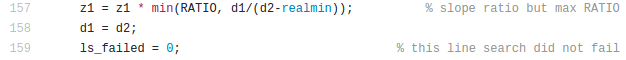
\includegraphics[width=\linewidth]{realmin.png}}
	\caption{MATLAB's \texttt{double} is actually a \texttt{float}? What it means for \texttt{realmin}.}
	\label{fig:realmin}
\end{figure}

Lastly, some of the optimisations in \texttt{fmincg} has been ignored, namely: (1) the innermost and middle loop iterations, thus the loop counter \texttt{M} is set to 1; and, (2) the handling of a failure case. The reason for (2) has already been discussed in \ref{se:impl.fmincg}. For (1), testing has shown that the iterations other than exactly once for the sections in question produces erroneous results, and the reasons for this is unfortunately still unknown at the time of writing. In addition, although setting \texttt{M=1} seems to closely align my program's results to MATLAB's results in the first training set, my neural network was unable to yield as high accuracy rate as in ~\cite{LeC98} for the second training set, almost off by 10 per cent (see Chapter~\ref{ch:results}).

\section{Other works}
I have also implemented a logistic regression cost function, which is akin to a neural network without any hidden layers. This can be accessed at ~\cite{McDJeo}.